\documentclass[11pt,a4paper]{article}
\usepackage[T1]{fontenc}
\usepackage[utf8]{inputenc}
\usepackage{lmodern}
\usepackage{amsmath}
\usepackage{amssymb}
\usepackage[margin=2.3cm]{geometry}
\usepackage{microtype}
\usepackage{booktabs}
\usepackage{tabularx}
\usepackage{graphicx}
\usepackage[font=small,labelfont=bf]{caption}
\usepackage{float}
\usepackage{enumitem}
\usepackage{xcolor}
\usepackage{fancyvrb}
\usepackage[colorlinks=true,linkcolor=blue!50!black,urlcolor=blue!50!black]{hyperref}

\setlist{nosep,leftmargin=*}
\setlength{\parskip}{0.5em}
\setlength{\parindent}{0pt}
\setlength{\emergencystretch}{3em}
\newcolumntype{Y}{>{\raggedright\arraybackslash}X}
\newcommand{\best}[1]{\textbf{#1}}
\newcommand{\code}[1]{\texttt{#1}}

\title{\textbf{IRWA Final Project --- Part 4}\\[0.2em]\large RAG, User Interface and Web Analytics}
\author{\begin{tabular}{ccc}Èric Amargant & Josep Cardona & Jan Balayla\\\small u231867 -- NIA 284566 & \small u231747 -- NIA 284888 & \small u233694 -- NIA 286572\end{tabular}}
\date{November 2026}

\begin{document}
\maketitle

\textbf{GitHub repository:} \url{https://github.com/Janbacer/irwa-search-engine}\\
\textbf{Tag:} \texttt{IRWA-2026-part-4}\\
The \code{README.md} in the main folder explains step by step how to install and run the web application and how to
choose the ranking algorithm and the other options. The README of this part
(\code{project\_progress/part\_4/README.md}) lists its files and how to reproduce the results of this report.

In this part our search engine becomes a web application (Flask): a search page, a results page with filters and an
AI summary (RAG), a details page for every product, and a web analytics module with a dashboard.
Figure~\ref{fig:arch} shows how the pieces fit together. Following the course template, the application is
\code{web\_app.py} and the package \code{myapp/} (\code{search}, \code{generation}, \code{analytics}); the evaluation
scripts, the result tables and the figures of this report are in \code{project\_progress/part\_4/}.

\begin{figure}[H]
\centering
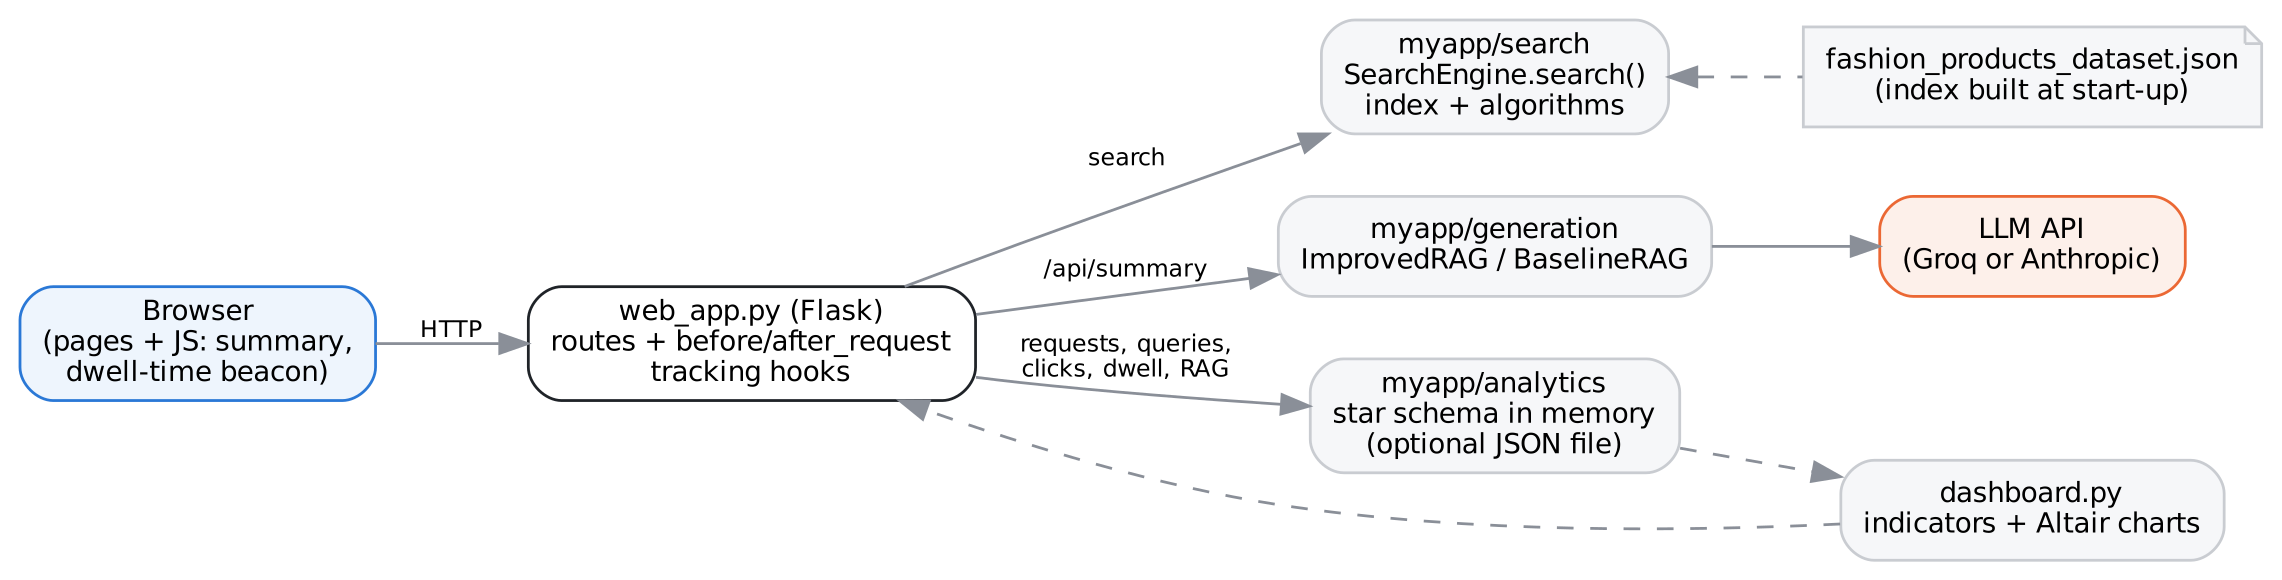
\includegraphics[width=\textwidth]{figures/architecture.png}
\caption{Architecture of the web application. Every request goes through the tracking hooks of Flask; the AI summary
is requested by the results page after it is shown, so the results never wait for the LLM.}
\label{fig:arch}
\end{figure}

%=====================================================================================================
\section{The search engine of the web application}
\label{sec:engine}

\subsection{One general search function}
The template only had a dummy search that returned random products. We rewrote our Part~1--3 code as a package that
the web application can use (\code{myapp/search}):

\begin{itemize}
\item \code{preprocessing.py}: the Part~1 text pipeline (the same function for products and queries);
\item \code{index.py}: \code{SearchIndex}, built once when the server starts from the JSON dataset (a few seconds for
the 28,080 products: about 4~seconds on our computers, including the product objects). It holds everything that does not
depend on the query;
\item \code{algorithms.py}: the four rankings of Part~3 (TF-IDF + cosine, BM25, our score, word2vec), with the same
formulas;
\item \code{search\_engine.py}: \code{SearchEngine.search(query, method, filters, sort, page, page\_size)}, the general
search function called by the results page.
\end{itemize}

The search function works in six steps: (1) it reads a price from the query, (2) it pre-processes the query, (3) it
finds the products with \emph{all} the query terms (conjunctive search, as in Parts~2--3), (4) if there are none, it
tries a spelling correction and then partial matches, (5) it applies the filters chosen by the user, and (6) it ranks
the products with the chosen algorithm (or sorts them by price, rating or discount) and returns one page of results.
It returns a \code{SearchResponse} with the results, the number of matches, the category counts, what happened
(full match, corrected, partial or none) and the time it took.

\textbf{Check against Part~3.} With the Part~1 pre-processing, the new code gives \emph{exactly} the same top~20 as the
Part~3 code for the five test queries and the four methods (20 of 20 rankings identical,
\code{results/reproduction\_part3.csv}), so the rewrite did not change the algorithms.

\subsection{Optimisations for a real use case}
The statement asks to optimise the algorithms now that there is a real use case: better results, faster, cleaner
and better suited to the user. We made five changes.

\textbf{1. Keeping the numbers (better results).} In Part~3 the query \emph{women pure cotton t-shirt pack of 3} lost
its ``3'' in the pre-processing, so no ranking could tell a pack of 3 from a pack of 5 (our score: NDCG@10 = 0.55 on
this query). Users type sizes and pack sizes, so the web engine keeps number tokens (also one-digit ones; the other
one-letter tokens are still removed). Q4 now has 26 AND matches instead of 140, exactly the 26 relevant products, and
every method gets NDCG@10 = 1.00 on it. Table~\ref{tab:numbers} shows the effect with the complete Part~3 labels: our
score reaches NDCG@10 = 0.98 and MRR = 1. The other queries have no numbers, so their set of matches is the same, but
the lengths and norms of the products change a little: TF-IDF gets worse on Q5 (0.51 $\to$ 0.22) and better on the
mean. The validation queries do not change (they have no numbers).

\begin{table}[H]
\centering\small
\caption{Effect of keeping the numbers: mean over the test queries Q1--Q5 (all AND matches judged, Part~3 labels).
\code{results/metrics\_test\_*.csv} also has $K = 5$ and $20$.}
\label{tab:numbers}
\begin{tabular}{@{}l cccc c cccc@{}}
\toprule
 & \multicolumn{4}{c}{Part 1 pre-processing (Part 3)} && \multicolumn{4}{c}{numbers kept (web app)}\\
\cmidrule(lr){2-5}\cmidrule(lr){7-10}
method & P@10 & MAP@10 & NDCG@10 & MRR && P@10 & MAP@10 & NDCG@10 & MRR\\
\midrule
TF-IDF + cosine & .580 & .628 & .617 & .680 && .680 & .698 & .701 & .680\\
BM25 & .460 & .793 & .605 & .900 && .560 & .864 & .698 & .900\\
Our score & .740 & .915 & .890 & 1.00 && \best{.840} & \best{.986} & \best{.982} & \best{1.00}\\
word2vec + cosine & .580 & .698 & .628 & .640 && .680 & .783 & .735 & .740\\
\bottomrule
\end{tabular}
\end{table}

\textbf{2. No dead ends (better suited to the user).} With a strict AND search a typo or one unknown word gives an
empty page. When no product has all the terms, the engine now (a) replaces the words that are not in the vocabulary by
the most likely word of the products (\code{difflib} similarity $\ge 0.75$ plus a small bonus for frequent words, so
that ``shrit'' becomes ``shirt'' and not the rare ``shrt''), and (b) if there is still nothing, shows the products
that contain the largest number of the query terms. The page always says which case happened
(Figure~\ref{fig:corrected}), so the user is not misled. Examples (\code{results/fallback\_examples.csv}):
\emph{black runing shoes for men} $\to$ \emph{black running shoes for men} (28 results);
\emph{jens blue men} $\to$ \emph{jeans blue men} (538); \emph{women floral sweatshirt hoodie zipper xyzzy} $\to$ the product
with 4 of the 6 words. The fallback is only used when the AND search finds nothing, so it never changes a query that
already works.

\textbf{3. Query understanding of prices.} A shopper writes ``cheap cotton shirt for men under 500''. ``Cheap'',
``under'' and ``500'' are not words of a product, so the AND search failed and the partial match returned running
shoes. The engine now reads price expressions (``under/below/up to $X$'', ``over/above $X$'', ``between $X$ and $Y$'',
with or without ``Rs''), turns them into a price filter, and drops words that describe the price and not the product
(``cheap'', ``budget''...). The query above becomes \emph{cotton shirt for men} with a maximum price of Rs~500: 519
shirts. The results page shows the filter it read from the query (Figure~\ref{fig:results}).

\textbf{4. Filters, sorting and pages.} The results page has filters on the structured fields of Part~1: category
(with the number of matches of each), price range, minimum rating, minimum discount and ``only in stock''; the results
can also be sorted by price, rating or discount (the score breaks the ties), and they are shown 20 per page. The
filters are applied to the AND matches, so they never add products that do not match the query.

\textbf{5. Speed.} In Part~3 the BM25F pseudo-frequency $\widetilde{tf}(t,d)$ of our score was recomputed for every
product at every query, although it does not depend on the query. The index now stores it for every (term, product)
pair, and the postings store the term frequencies, so a search only reads numbers and adds them. Table~\ref{tab:speed}
compares the median time per search (20 runs) of the Part~3 code and of the web engine, with the same pre-processing
and the same results. For our score the web engine is 2.4--4.2 times faster, including the time
to build the result records of the page. For TF-IDF and BM25 on broad queries (thousands of matches) the gain is small:
most of the time is now sorting the matches, which both versions do. Every search of the test queries takes
0.9--3.0~ms.

\begin{table}[H]
\centering\small
\caption{Median time per search in milliseconds (\code{results/speed.csv}; the web-app time includes the result
records of the page). Same computer, same results.}
\label{tab:speed}
\begin{tabular}{@{}lr rrr rrr@{}}
\toprule
 & & \multicolumn{3}{c}{Part 3 code} & \multicolumn{3}{c}{web app}\\
\cmidrule(lr){3-5}\cmidrule(lr){6-8}
query & matches & TF-IDF & BM25 & ours & TF-IDF & BM25 & ours\\
\midrule
Q1 men white formal shirt slim fit & 25 & 6.6 & 7.6 & 6.1 & 1.9 & 1.8 & 1.8\\
Q4 women pure cotton t-shirt pack of 3 & 140 & 17.4 & 10.8 & 12.5 & 2.8 & 2.9 & 3.0\\
black jeans & 589 & 3.4 & 3.7 & 5.3 & 2.5 & 1.7 & 2.0\\
shirt & 4,813 & 11.9 & 10.4 & 37.9 & 9.9 & 9.6 & 14.1\\
women tshirt & 6,786 & 25.1 & 28.8 & 89.9 & 19.6 & 23.0 & 33.7\\
men & 14,233 & 40.4 & 46.2 & 132.3 & 41.0 & 51.1 & 50.9\\
\bottomrule
\end{tabular}
\end{table}

The default ranking of the web application is our score, the best one in Part~3 and again here. The other three can
be chosen on the search and results pages (or with the URL parameter \code{method}); word2vec is trained on its first
use (about 30~s) because most users never choose it.

%=====================================================================================================
\section{User interface}
\label{sec:ui}

\textbf{Search page} (\code{/}, Figure~\ref{fig:home}): a central search box with a button, the choice of the ranking
algorithm and a few example queries. The form sends a GET request (\code{/search?q=...}), so a results page has its
own URL: it can be reloaded, shared or opened again with the browser's back button. The POST form of the template is
still accepted and redirected.

\begin{figure}[H]
\centering
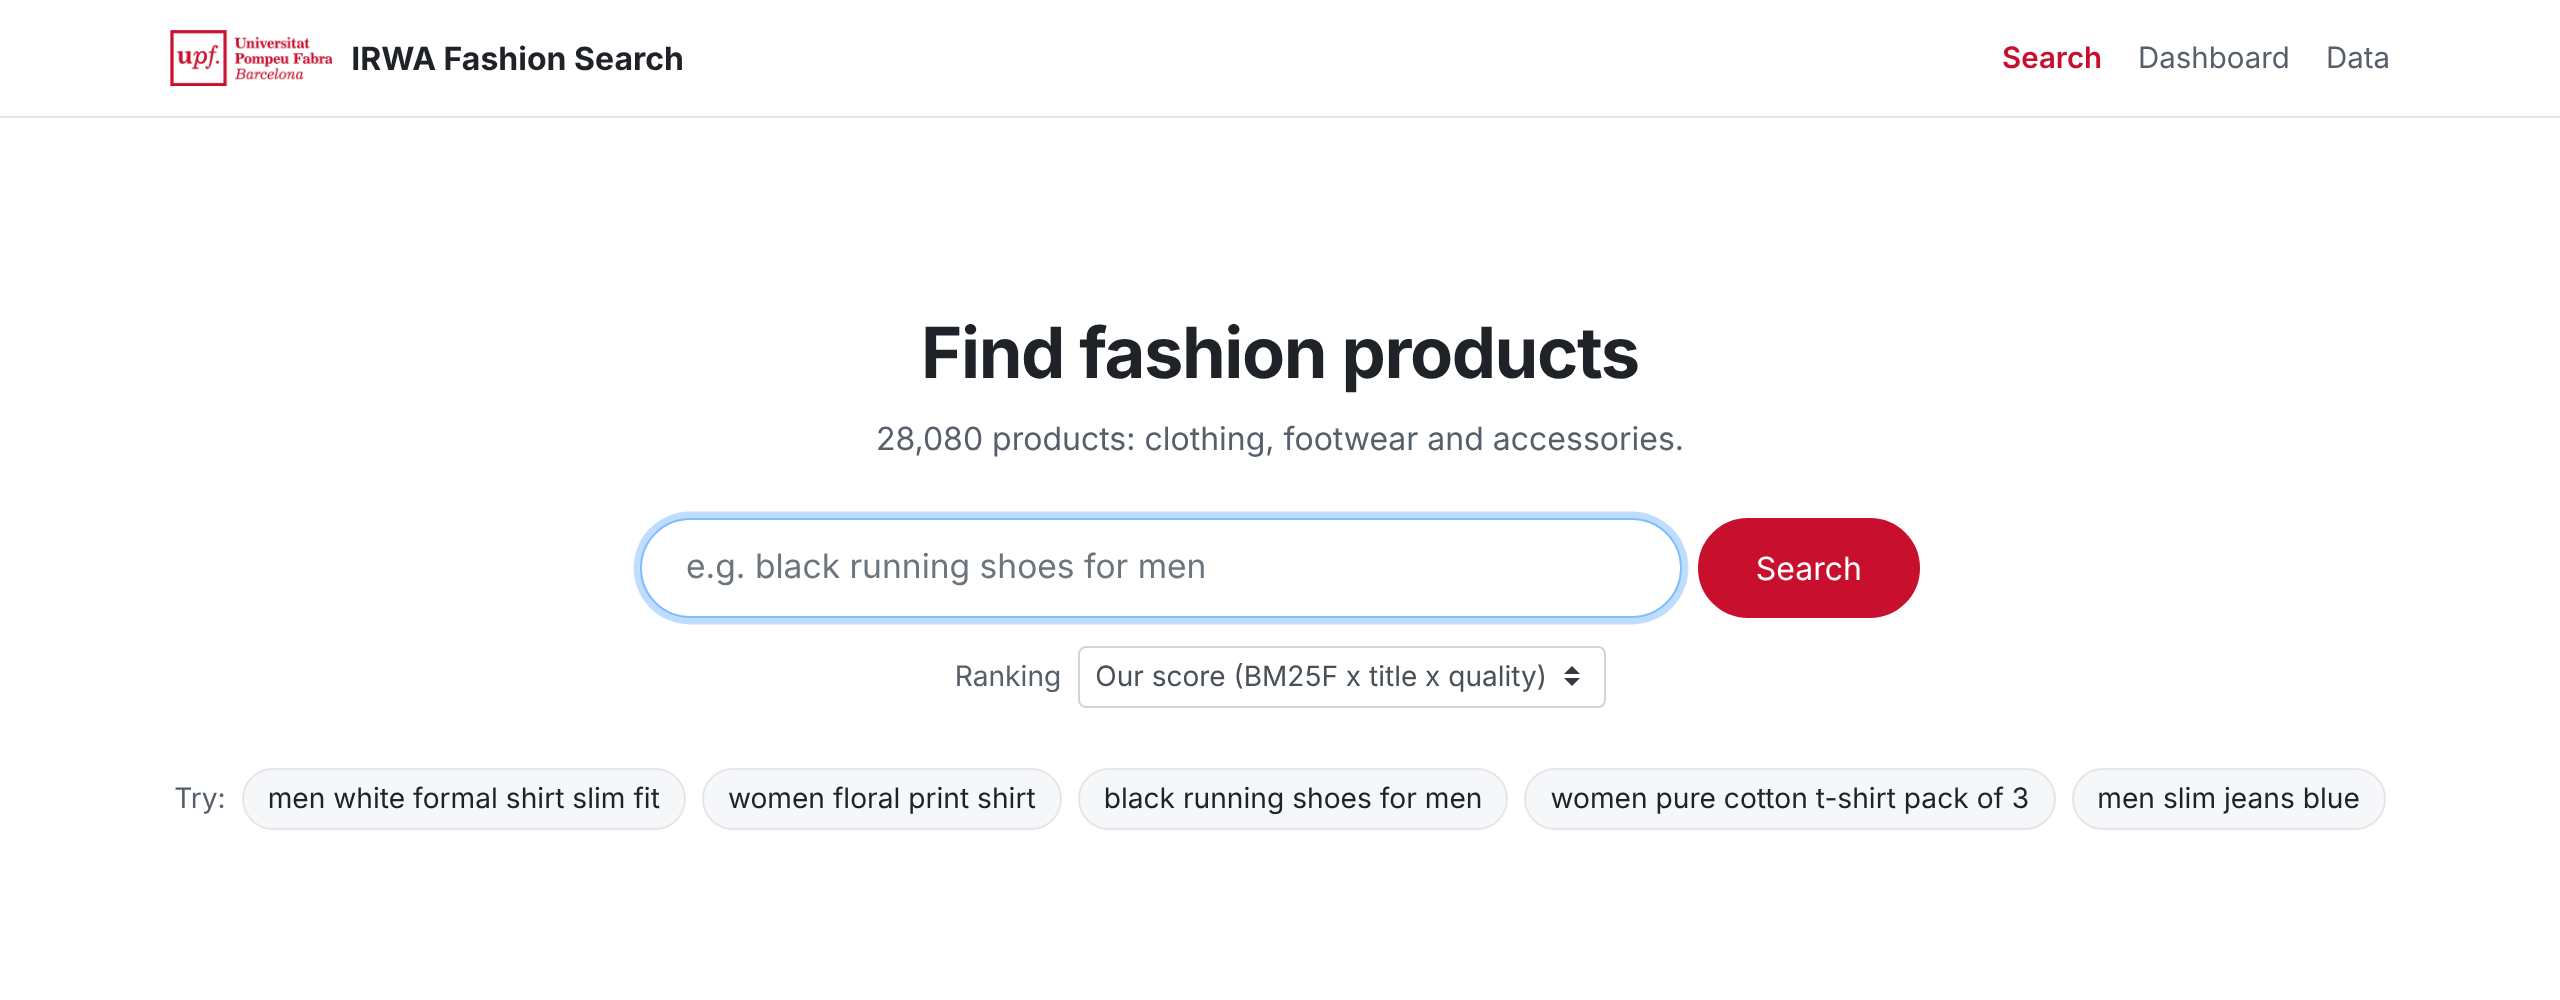
\includegraphics[width=0.85\textwidth]{figures/ui_home.png}
\caption{Search page.}
\label{fig:home}
\end{figure}

\textbf{Search action and results page} (\code{/search}, Figure~\ref{fig:results}). The query is passed to
the general search function (\code{SearchEngine.search}) with the chosen algorithm, filters, sorting and page. Each result shows the title (link to
the details page), brand, category, colour, average rating, stock, selling price with the original price and the
discount, the start of the description, a link to the product on the original website, and its rank, score and PID
(useful to check the ranking). We also show the first image of the product, loaded from the original website. The
head of the page gives the number of results (and before filters) and the search time; a notice explains a spelling
correction, a partial match or a price read from the query (Figure~\ref{fig:corrected}).

\begin{figure}[H]
\centering
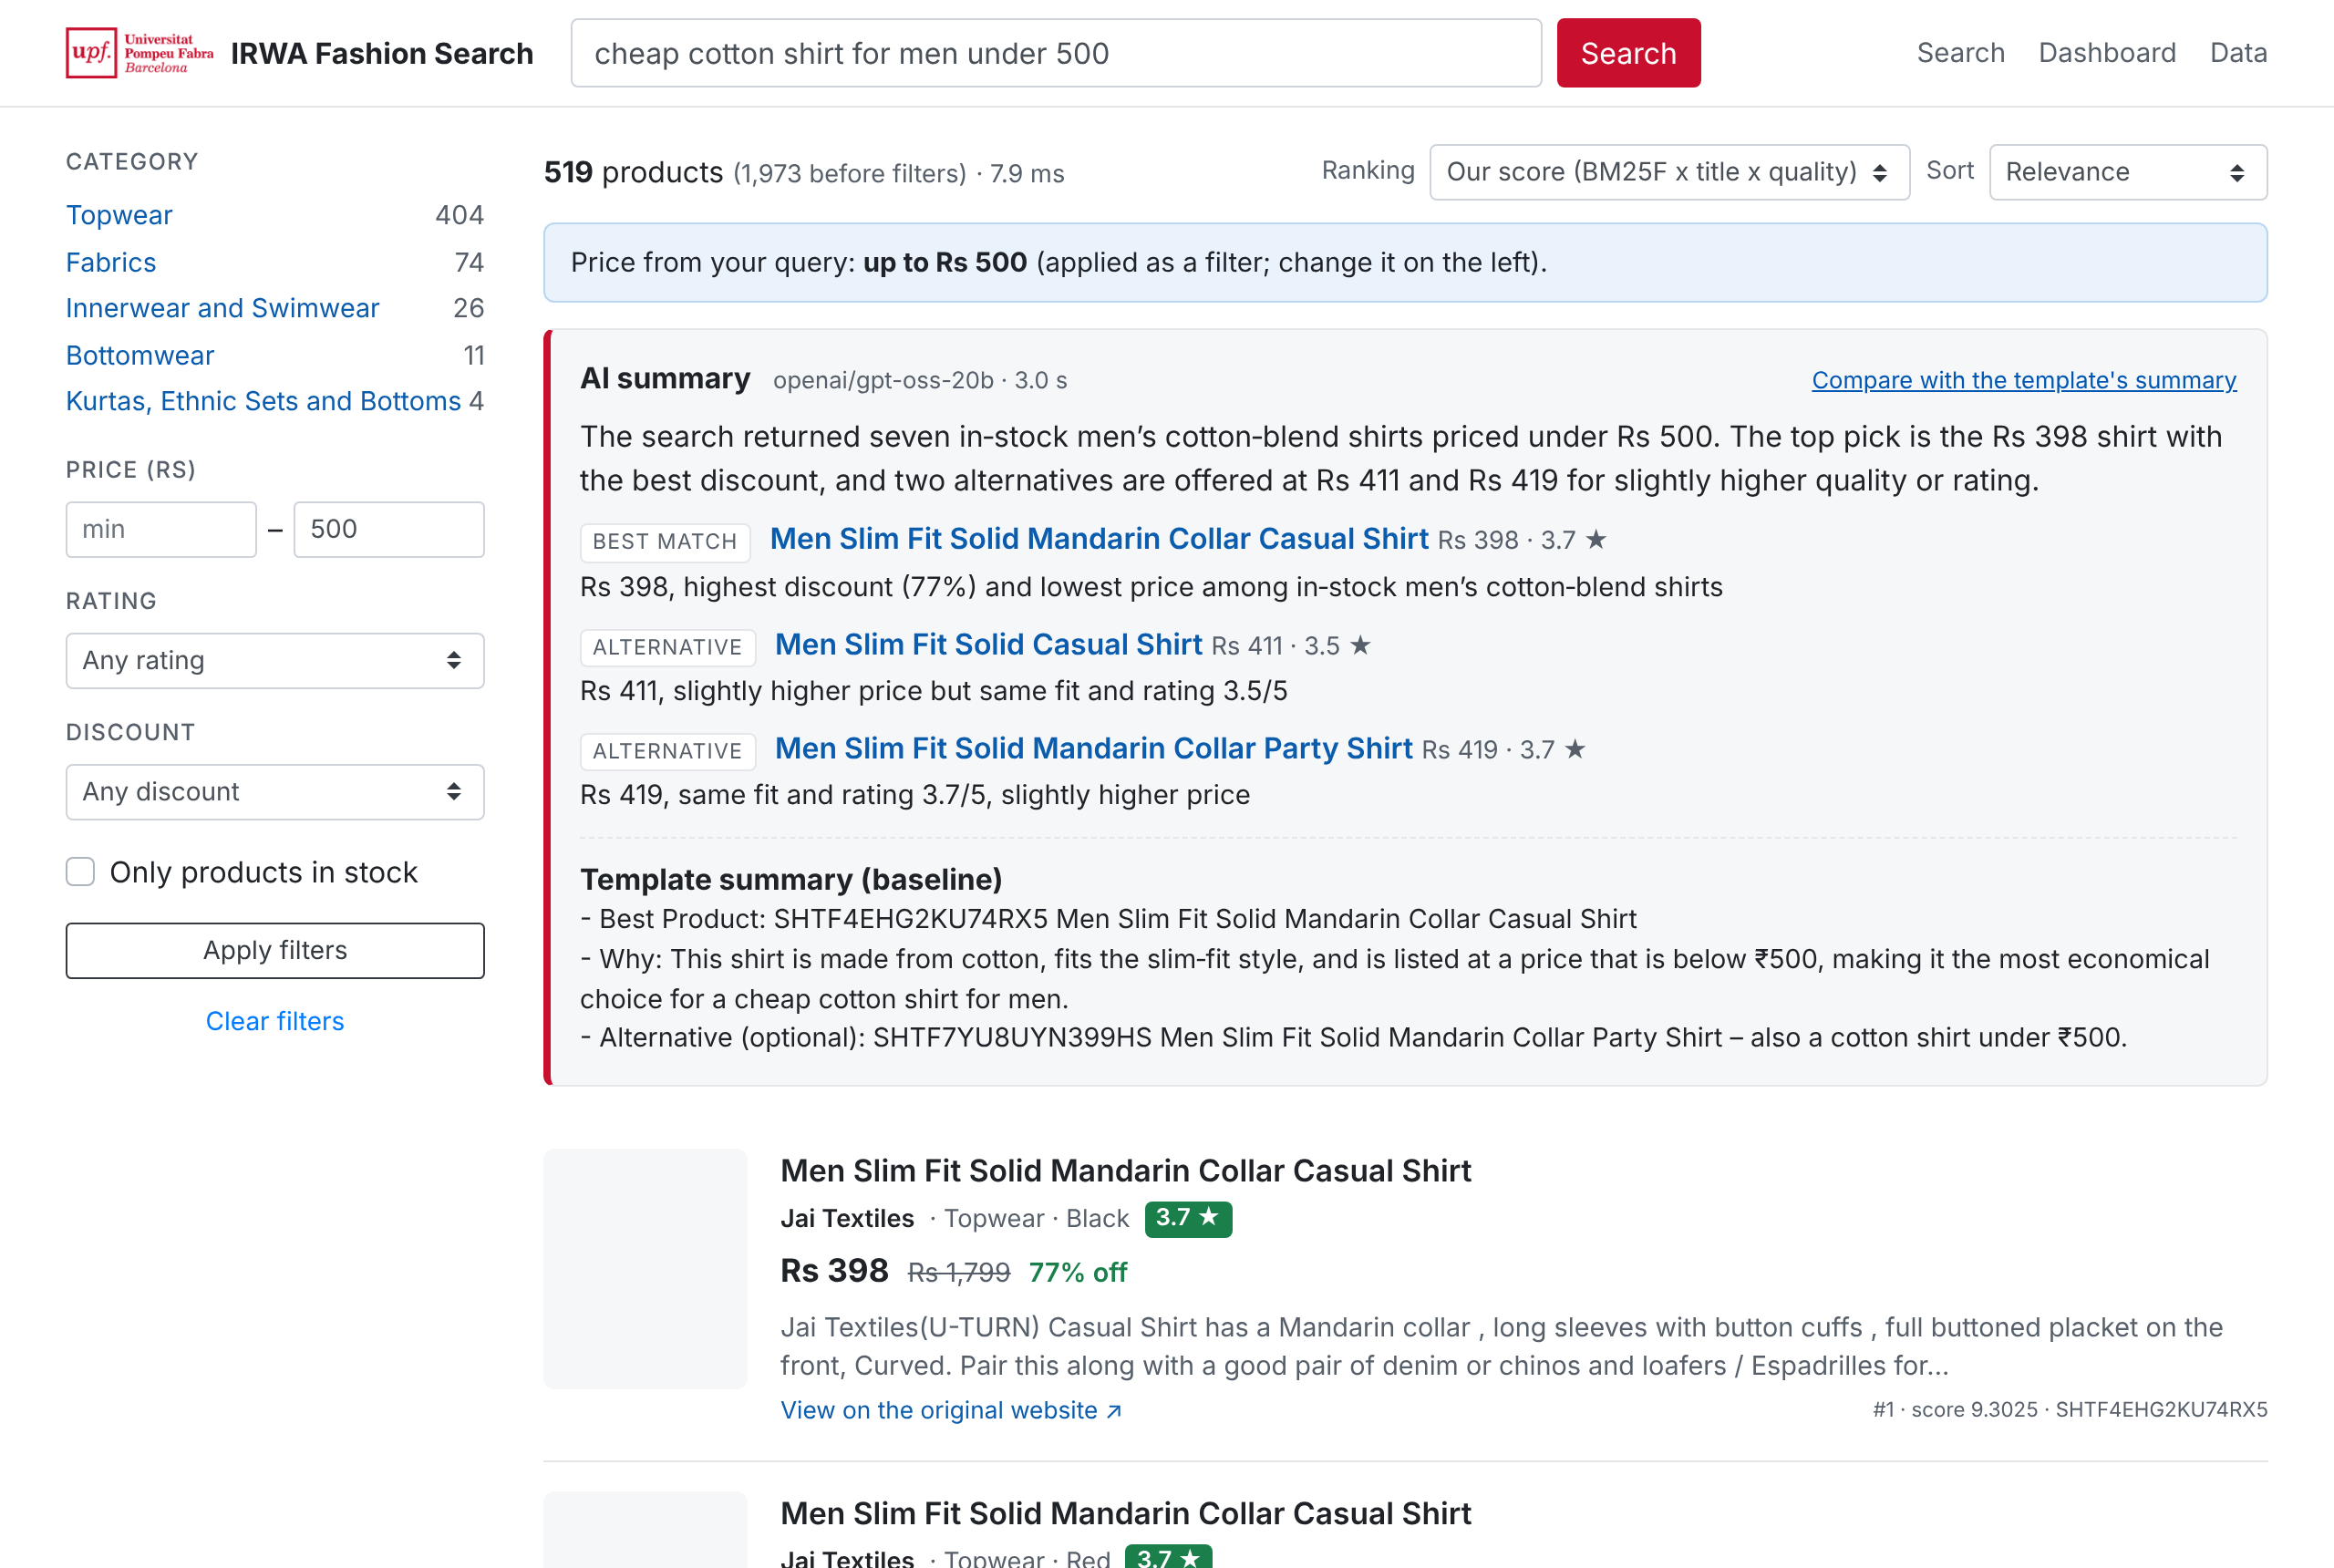
\includegraphics[width=\textwidth]{figures/ui_results.png}
\caption{Results page for \emph{cheap cotton shirt for men under 500}: the price was read from the query and applied
as a filter. The AI summary (our RAG, with the template's summary opened below it for comparison) shows the answers of
\code{openai/gpt-oss-20b} recorded in our evaluation run (Section~\ref{sec:rag}). The images of the products are
loaded from the original website; they could not be loaded in the environment where we took the screenshots, so the
boxes are empty.}
\label{fig:results}
\end{figure}

\begin{figure}[H]
\centering

\includegraphics[width=\textwidth]{figures/ui_corrected.png}
\caption{A query with a typo: the page says which query was used.}
\label{fig:corrected}
\end{figure}

\textbf{LLM summary.} In the template the LLM was called inside the search request, so the results page waited for
the LLM (1--3~s with a fast model, and the whole page failed if the API was slow). Our results page appears at once
and loads the summary from \code{/api/summary} with a few lines of JavaScript; the box shows a spinner meanwhile. A
link shows the summary of the template's pipeline next to ours, to compare them (Section~\ref{sec:rag}).

\textbf{Details page} (\code{/doc/<pid>}, Figure~\ref{fig:details}): every field of the product: the images, title,
category and sub-category, brand (the cut field of the dataset and the full name recovered from the URL in Part~1),
seller, selling and actual price, discount, rating, stock, crawl date, PID and URL, the full description and the table
of product details. A clicked result reaches it with its query and rank in the URL (\code{?qid=...\&rank=...}), which
is how the click is recorded (Section~\ref{sec:analytics}).

\begin{figure}[H]
\centering
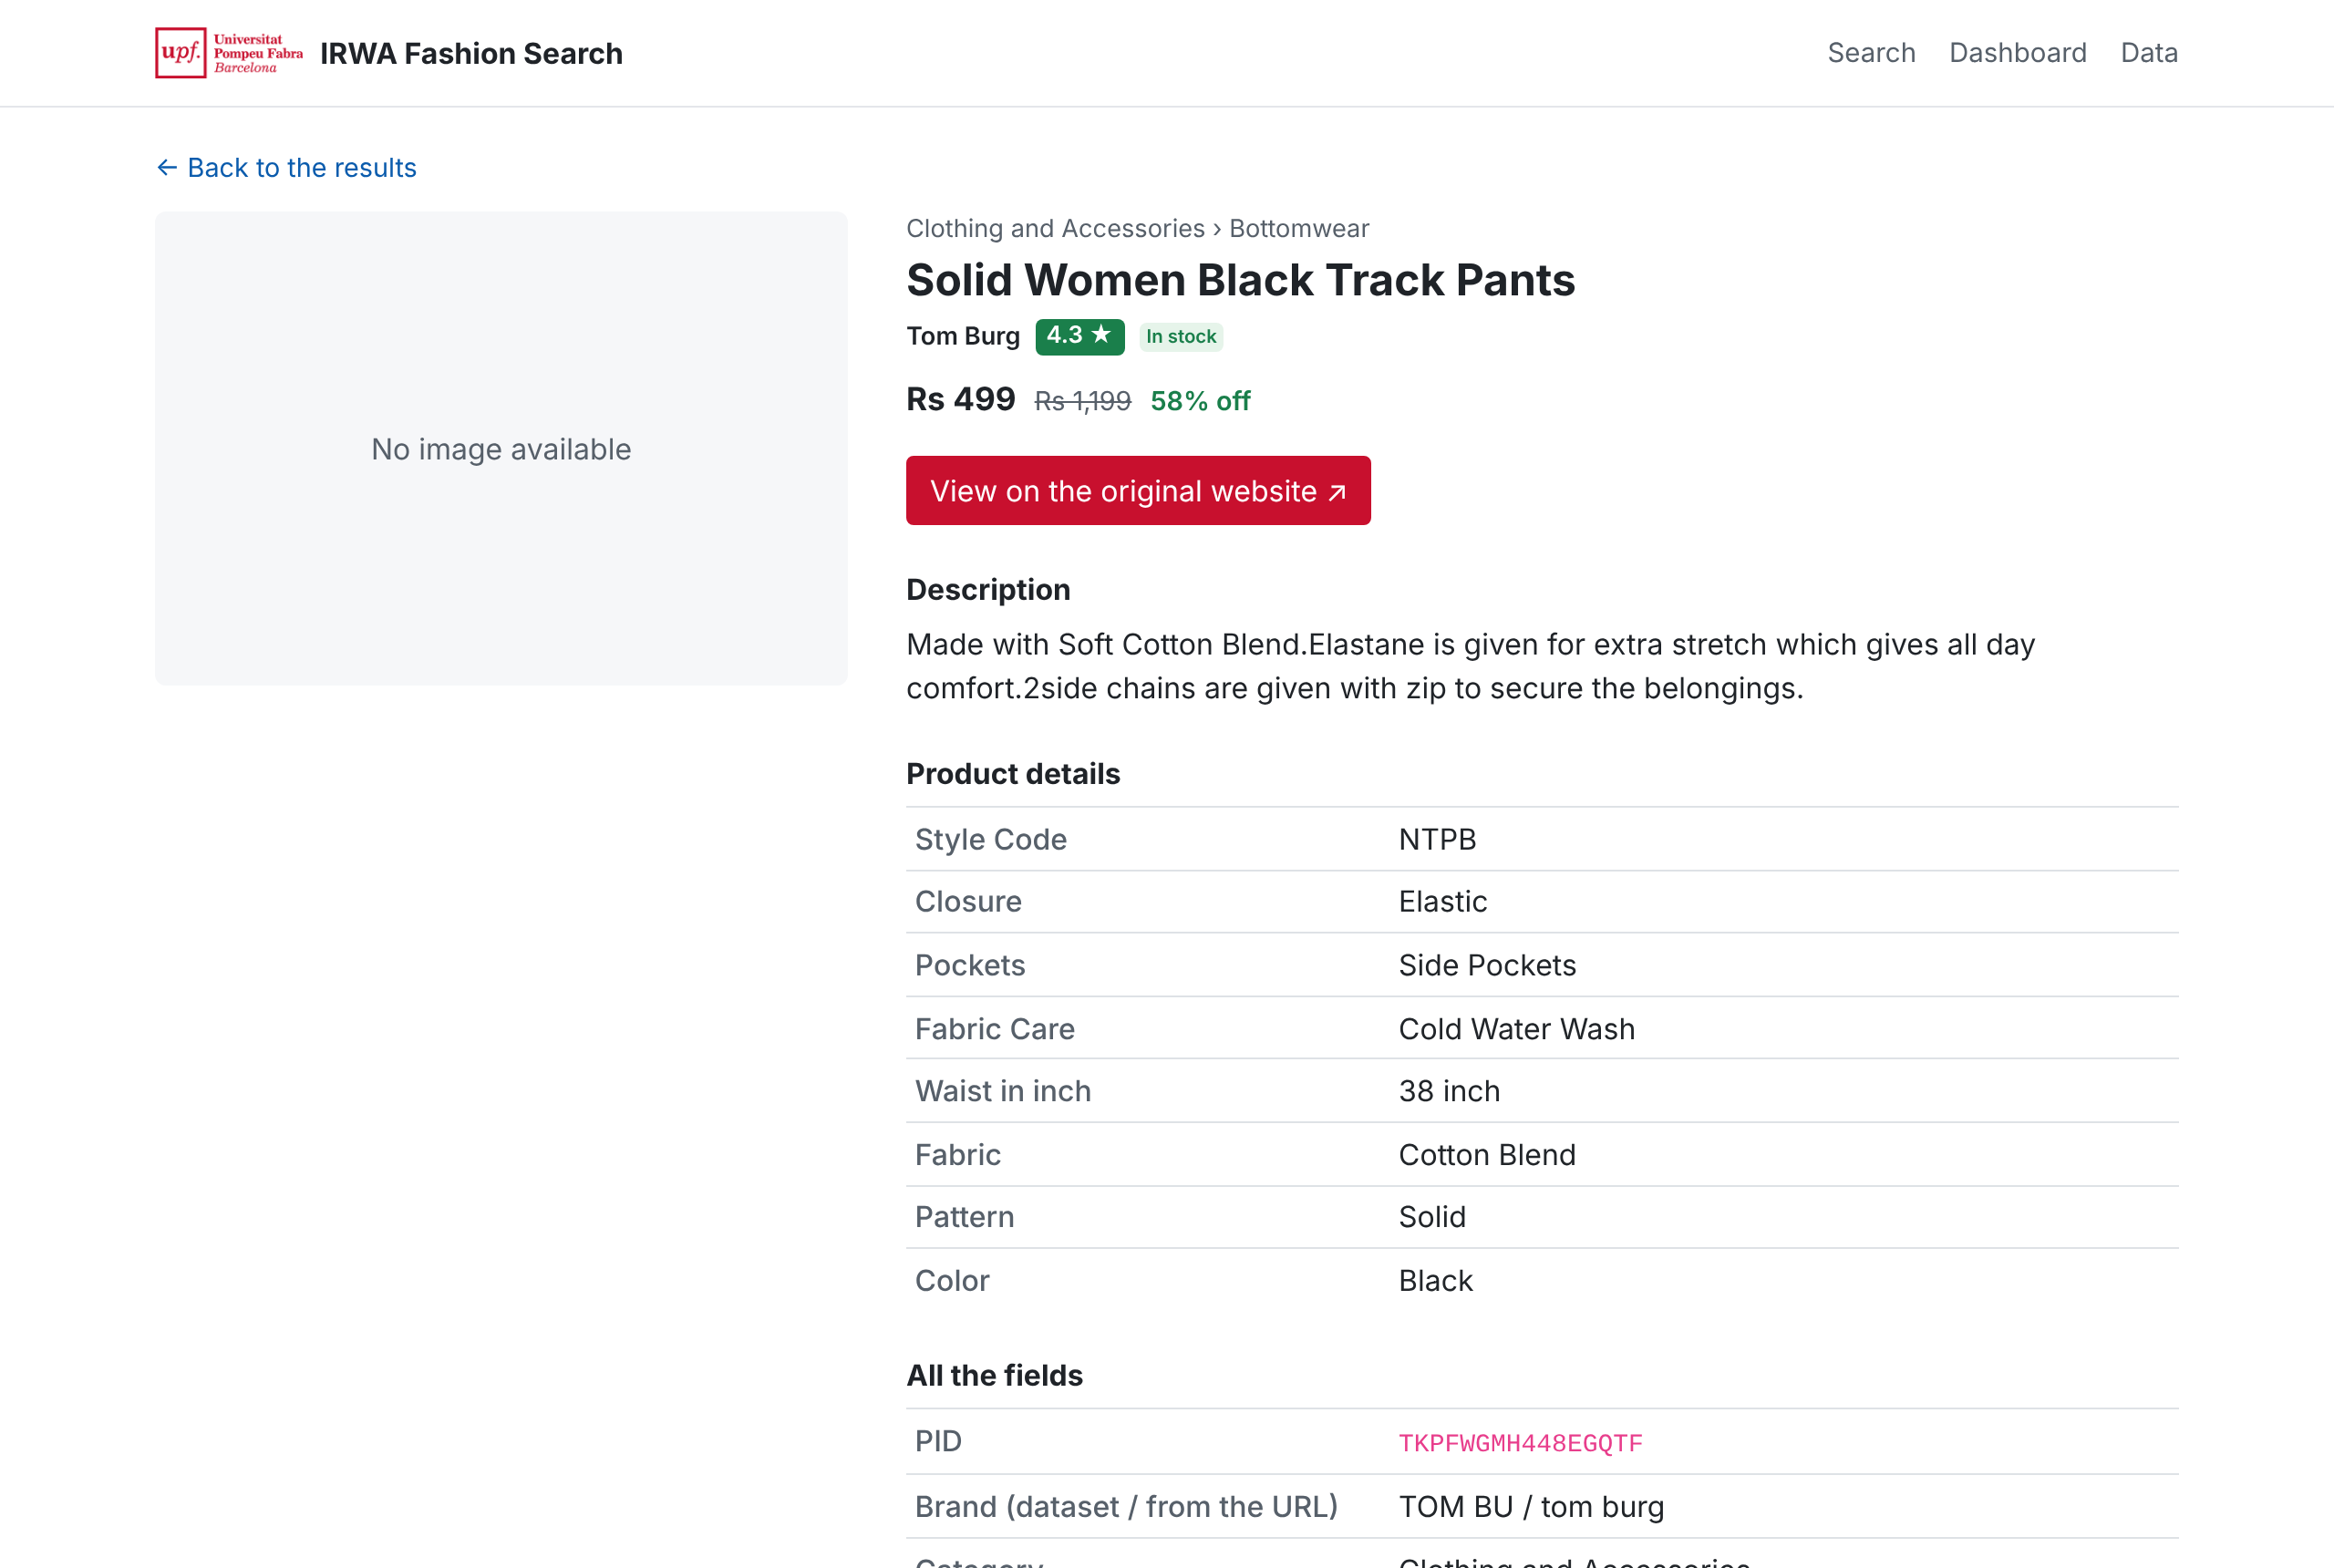
\includegraphics[width=0.92\textwidth]{figures/ui_details.png}
\caption{Details page of a product (top part), reached from the first result of
\emph{women black track pants with zip pockets}.}
\label{fig:details}
\end{figure}

%=====================================================================================================
\section{RAG: from the baseline to our version}
\label{sec:rag}

The course template gives a basic RAG (\code{myapp/generation/rag.py}): the PID and title of the top~20 results are
put in a prompt that asks for the best product, a reason and an alternative, or a fixed sentence if no product fits.
We kept it unchanged as \code{BaselineRAG} and wrote \code{ImprovedRAG}. Both use the same retrieval (our search
engine) and the same LLM, so the comparison only measures the generation. The LLM is reached through a third-party
API: Groq, as in the template, or Anthropic, chosen in \code{.env}. The template's model, \code{llama-3.1-8b-instant},
is no longer offered by Groq, so our default is \code{openai/gpt-oss-20b}, the smallest general model available there
(an open-weight reasoning model; we use it with low reasoning effort).

\subsection{Weaknesses of the baseline}
\begin{enumerate}
\item \textbf{The model only sees titles.} The prompt asks to explain the choice with ``price, features, quality'',
but none of these is in the context: the model either guesses them (hallucination) or gives generic reasons. Many titles
do not even include the colour (the title ``Men Slim Fit Solid Mandarin Collar Casual Shirt'' belongs to 41 products of
9 brands in 15 colours), and none says whether the product is in stock.
\item \textbf{Twenty near-identical lines.} The same product in several colours or sizes has the same title, so the
top~20 often contains the same line many times. It is a long prompt with little information.
\item \textbf{Free text that cannot be checked.} The answer is a text in an informal format: the code cannot verify
that the recommended PID was really retrieved (a model can invent or mistype a PID), and the page cannot turn the
recommendation into a link.
\item \textbf{``No good products'' only as an instruction.} The search can return products that do not fit (a
partial match, or a product that only mentions the query word), and small models tend to recommend something anyway.
When the search finds nothing, the template still calls the LLM with an empty list.
\item \textbf{No system message and the default temperature}, so the answers vary from one run to another.
\end{enumerate}

\subsection{Our three improvements}

\textbf{1. A richer and smaller context.} For each product we give the facts a shopper decides on: title, brand,
price (and the original price and discount), rating, stock, category, the key product details (colour, fabric, fit,
pattern, occasion, ideal for, pack size...) and the first 200 characters of the description. We give the top~8
products instead of~20, and we skip near-duplicates (same title, brand and price), filling the 8 places from the
top~20.
\emph{Why it helps:} the model can check the requirements of the query (``black'', ``for men'', ``pack of 3'') and
explain its choice with real facts. \emph{Pros:} grounded explanations; the products are more varied.
\emph{Cons:} a longer prompt (about twice as many characters), so more tokens and a little more time; with only 8
products, a good product at rank 12 is not considered (it relies on the ranking being good, which our score is).

\textbf{2. A grounded, structured prompt.} A system message sets the rules: use only the listed products, never invent
products, PIDs, prices or features. The task is written step by step: list the explicit requirements of the request,
keep only the products that meet all of them, choose the best (in stock first; rating, price and discount only to
break ties), up to two alternatives, and a two-sentence summary. The answer must be a JSON object, and the temperature
is 0.2.
\emph{Why it helps:} the steps make the model check the constraints instead of picking the first title; JSON can be
parsed, checked and shown as links; a low temperature gives stable answers. \emph{Pros:} the page shows the best product
and the alternatives as cards with links, price and rating (Figure~\ref{fig:results}). \emph{Cons:} JSON mode may fail
with some models (we then show the text, but do not trust it as a recommendation); stricter instructions may make the
model refuse more often.

\textbf{3. Handling ``no good products'' before and after the LLM.}
\begin{itemize}
\item \emph{Before}: if the search finds nothing, the LLM is not called and the page says so (no cost, no invented
answer). If the results are a partial match or a corrected query, the prompt says it (``these products contain only 3
of the 5 key words of the request''), so the model knows they may not fit; the same for a price read from the query.
\item \emph{After}: every PID in the JSON answer is checked against the products given to the model. An unknown PID is
removed; if the best product is removed, the best valid alternative takes its place; with no valid product left, the
answer becomes ``no good products''.
\end{itemize}
\emph{Why it helps:} an invented product can never reach the user, and the model gets the information it needs to say
``nothing fits''. \emph{Pros:} safe by construction, cheaper when there is nothing to summarise. \emph{Cons:} the check
is on the PIDs, not on every sentence (a wrong fact about a real product is still possible, although the context makes
it less likely).

\subsection{Evaluation}
We compared both pipelines on 16 queries (\code{project\_progress/part\_4/evaluate\_rag.py}), with the same search
results (our score) and the same model (\code{openai/gpt-oss-20b} on Groq, 26/11/2026). Every answer is saved in
\code{results/rag\_comparison.json} and \code{.md}. The queries are of three kinds:
\begin{itemize}
\item \textbf{labelled}: Q1--Q5 and V1--V2, and T1, the typo ``black runing shoes for men'' (same need as Q5). Relevant
products are always retrieved, so ``no good products'' is a wrong answer. For Q1--Q5 and T1 every retrieved product has a
label, so we also know whether the recommended product is relevant (for V1--V2 only 20 products are judged);
\item \textbf{absent}: products the shop does not sell (``men leather wallet'', ``women high heels'', ``kids school
bag'', ``wedding saree'', ``laptop backpack''); the right answer is ``no good products'';
\item \textbf{open}: realistic needs without labels (``gift for my father'', ``comfortable shoes for walking'', ``cheap
cotton shirt for men under 500''), which we read.
\end{itemize}

\begin{table}[H]
\centering\small
\caption{Baseline (template) and improved RAG on the same 16 queries and the same model
(\code{results/rag\_summary.csv}, computed by code from the saved answers).}
\label{tab:rag}
\begin{tabularx}{\textwidth}{@{}Yrr@{}}
\toprule
 & baseline & ours\\
\midrule
relevant product recommended (Q1--Q5, T1) & 4 / 6 & \best{6 / 6}\\
wrong ``no good products'' although relevant products were retrieved (8 labelled queries) & 3 / 8 & \best{0 / 8}\\
correct ``no good products'' for products the shop does not sell & 5 / 5 & 5 / 5\\
answers with an invented PID & 0 / 16 & 0 / 16\\
prices, ratings and discounts in the explanations that match the product data & -- (not in its prompt) & 68 / 68\\
LLM calls & 16 & 15\\
median time of an answer & 2.3 s & 2.6 s\\
median prompt length (characters) & 2,392 & 4,517\\
\bottomrule
\end{tabularx}
\end{table}

\textbf{The baseline cannot check the requirements.} It answered ``no good products'' for Q3 (8 relevant products
retrieved), Q4 (26) and V1, because the titles do not say ``zip pockets'', ``pure cotton'' or ``cotton'': with titles only,
a careful model cannot verify the request, so it refuses. Our context has the product details and the description, so our
version found a relevant product for all six fully labelled queries:

\begin{quote}\small
\textbf{Q3} \emph{women black track pants with zip pockets}.\\
\textbf{Baseline}: ``There are no good products that fit the request based on the retrieved results.''\\
\textbf{Ours}: best match \emph{Solid Women Black Track Pants} (rank~1): ``from tom burg with a 58\% discount, priced at
Rs~499, and a 4.3/5 rating. It includes side zip pockets for secure storage.'' Two alternatives (Rs~765 and Rs~740).
Summary: ``The search returned several black track pants with zip pockets. The top pick is the most affordable with a
solid rating, while the alternatives offer slightly higher prices or a different color option.''
\end{quote}

\textbf{Grounded explanations.} Every price, rating and discount written in our explanations (68 numbers) is correct,
checked by code against the data. The baseline's reasons are generic or guessed: for Q1 it praises the ``breathable
fabric'' of a shirt whose fabric it never saw, and for \emph{cheap cotton shirt for men under 500} it says the shirt ``is
listed at a price that is below [Rs] 500'' without having any price in its prompt (it is true only because our search had
already applied the price filter). Ours gives the facts and the trade-off:

\begin{quote}\small
\textbf{O3} \emph{cheap cotton shirt for men under 500}. \textbf{Ours}: best match \emph{Men Slim Fit Solid Mandarin
Collar Casual Shirt}: ``Rs 398, highest discount (77\%) and lowest price among in-stock men's cotton-blend shirts'';
alternatives at Rs~411 and Rs~419. (The fabric of this shirt is indeed \emph{Cotton Blend}.)
\end{quote}

\textbf{``No good products''.} Both versions refuse the five products the shop does not sell. Ours says what the search
found instead (``The search returned a pair of suspenders, not a leather wallet''), and for \emph{laptop backpack},
with no result at all, it does not call the LLM. No answer contained an invented PID, so our PID check was never needed in
this run; it remains a guarantee for weaker models or longer contexts.

\textbf{Cost.} Our prompt is about twice as long, but the time of an answer is similar (the median is 2.6~s against
2.3~s; it varies more with the load of the API than with the prompt), and the results page does not wait for it.

\textbf{What is still wrong.} Our version is not perfect: for \emph{kids school bag} its summary over-generalises (``the
shop currently offers only raincoats and men's footwear'', when it only saw the top products), for V1 it says that
``one product matches all your criteria'' while other sweatshirts did too, and it often prefers a lower-ranked product with
a better rating (rank~6 for Q4 and Q5), which follows our instructions but means that the summary and the ranking do not
always agree. A larger model or a check of the summary sentence would reduce these errors.


%=====================================================================================================
\section{Web analytics}
\label{sec:analytics}

\subsection{Data collection}
Every request goes through two Flask hooks (\code{before\_request} and \code{after\_request} in \code{web\_app.py});
the pages add what only they know (the search, the click, the dwell time). Table~\ref{tab:collect} lists what we
collect, how, and why.

\begin{table}[H]
\centering\small
\caption{What the web application collects.}
\label{tab:collect}
\begin{tabularx}{\textwidth}{@{}>{\raggedright}p{3.0cm}YY@{}}
\toprule
data & how & why\\
\midrule
HTTP requests & every request except static files and dwell-time beacons: time, path, endpoint, method, status, server
time, referrer & traffic,
errors (status) and speed of the server\\
visitor & a random id in a cookie kept one year & returning visitors, research missions across days\\
physical session & a session id in Flask's signed session cookie; a new one after 30~min without requests & time-based
sessions (``sit-downs''), session length, bounce rate\\
user context & User-Agent $\to$ browser, OS and device (computer, mobile, tablet, bot); IP address; date and hour;
country and city from the IP (bonus) & who uses the site and how (mobile share, hours of use)\\
queries & text, terms after pre-processing, number of terms, order in the session, algorithm, sorting, filters,
page, outcome (full / corrected / partial / no match), number of results, search time & what people look for, failed
searches, which algorithm is used\\
missions & a query continues the current mission if it shares a non-common term with it, else it starts a new one;
a mission that shares a term with a mission of an earlier session of the same visitor continues its research mission
& logical sessions (bonus): how many searches a need takes\\
clicks on results & the details page receives the query id, rank and page in its URL & click-through rate, position
bias, which products attract\\
dwell time & the details page measures how long it is visible and sends it with \code{navigator.sendBeacon} when the
user leaves; if no beacon arrives, the time until the next request of the session is used & satisfaction: a short
click means the result did not fit\\
outbound clicks & the link to the original website goes through \code{/go/<pid>} & the clicks that lead to a purchase
on the shop\\
RAG summaries & variant, model, outcome, time, number of products, valid and invalid PIDs & cost and quality of the
RAG in use\\
\bottomrule
\end{tabularx}
\end{table}

Some choices need a justification. \emph{Common terms}: terms that appear in more than 20\% of the products, such as
``men'' or ``women'', do not link two queries into one mission (``men jeans'' and ``men shoes'' are different needs).
\emph{Dwell time}: the server alone cannot see when the user comes back, because the back button often shows the
results page from the browser's cache without a request; the beacon measures the time the page was really visible.
Dwell times over 30~minutes are cut, because they mean that the user left. \emph{Place}: country and city come from
the free service ip-api.com, looked up once per session; local addresses (such as 127.0.0.1 when the app runs on a
laptop) are reported as ``Local network'' without a look-up, and \code{GEOIP\_ENABLED=0} turns it off.
\emph{Privacy}: we store the IP address because the statement asks for it; a real deployment would need the user's
consent (cookie banner) and would store only a truncated IP.

\subsection{Data model}
We store the data as a star schema (Figure~\ref{fig:star}): the \emph{fact} tables hold the events (requests,
queries, clicks, RAG summaries) and point to the \emph{dimension} tables that describe them (visitors, sessions, and
the products, which are the corpus itself, by PID); the time dimension is derived from the timestamps (date, hour,
weekday). Clicks also point to their query, so a click can be analysed with the query that produced it (rank,
algorithm, filters). The tables are lists of Python dataclasses in memory (\code{myapp/analytics/analytics\_data.py}),
as the statement allows; \code{/stats} shows them and exports them as CSV or JSON. As an option, if \code{ANALYTICS\_FILE}
is set in \code{.env}, they are saved to that JSON file after each change and loaded when the server starts, so they
survive a restart (no database server to install).

\begin{figure}[H]
\centering
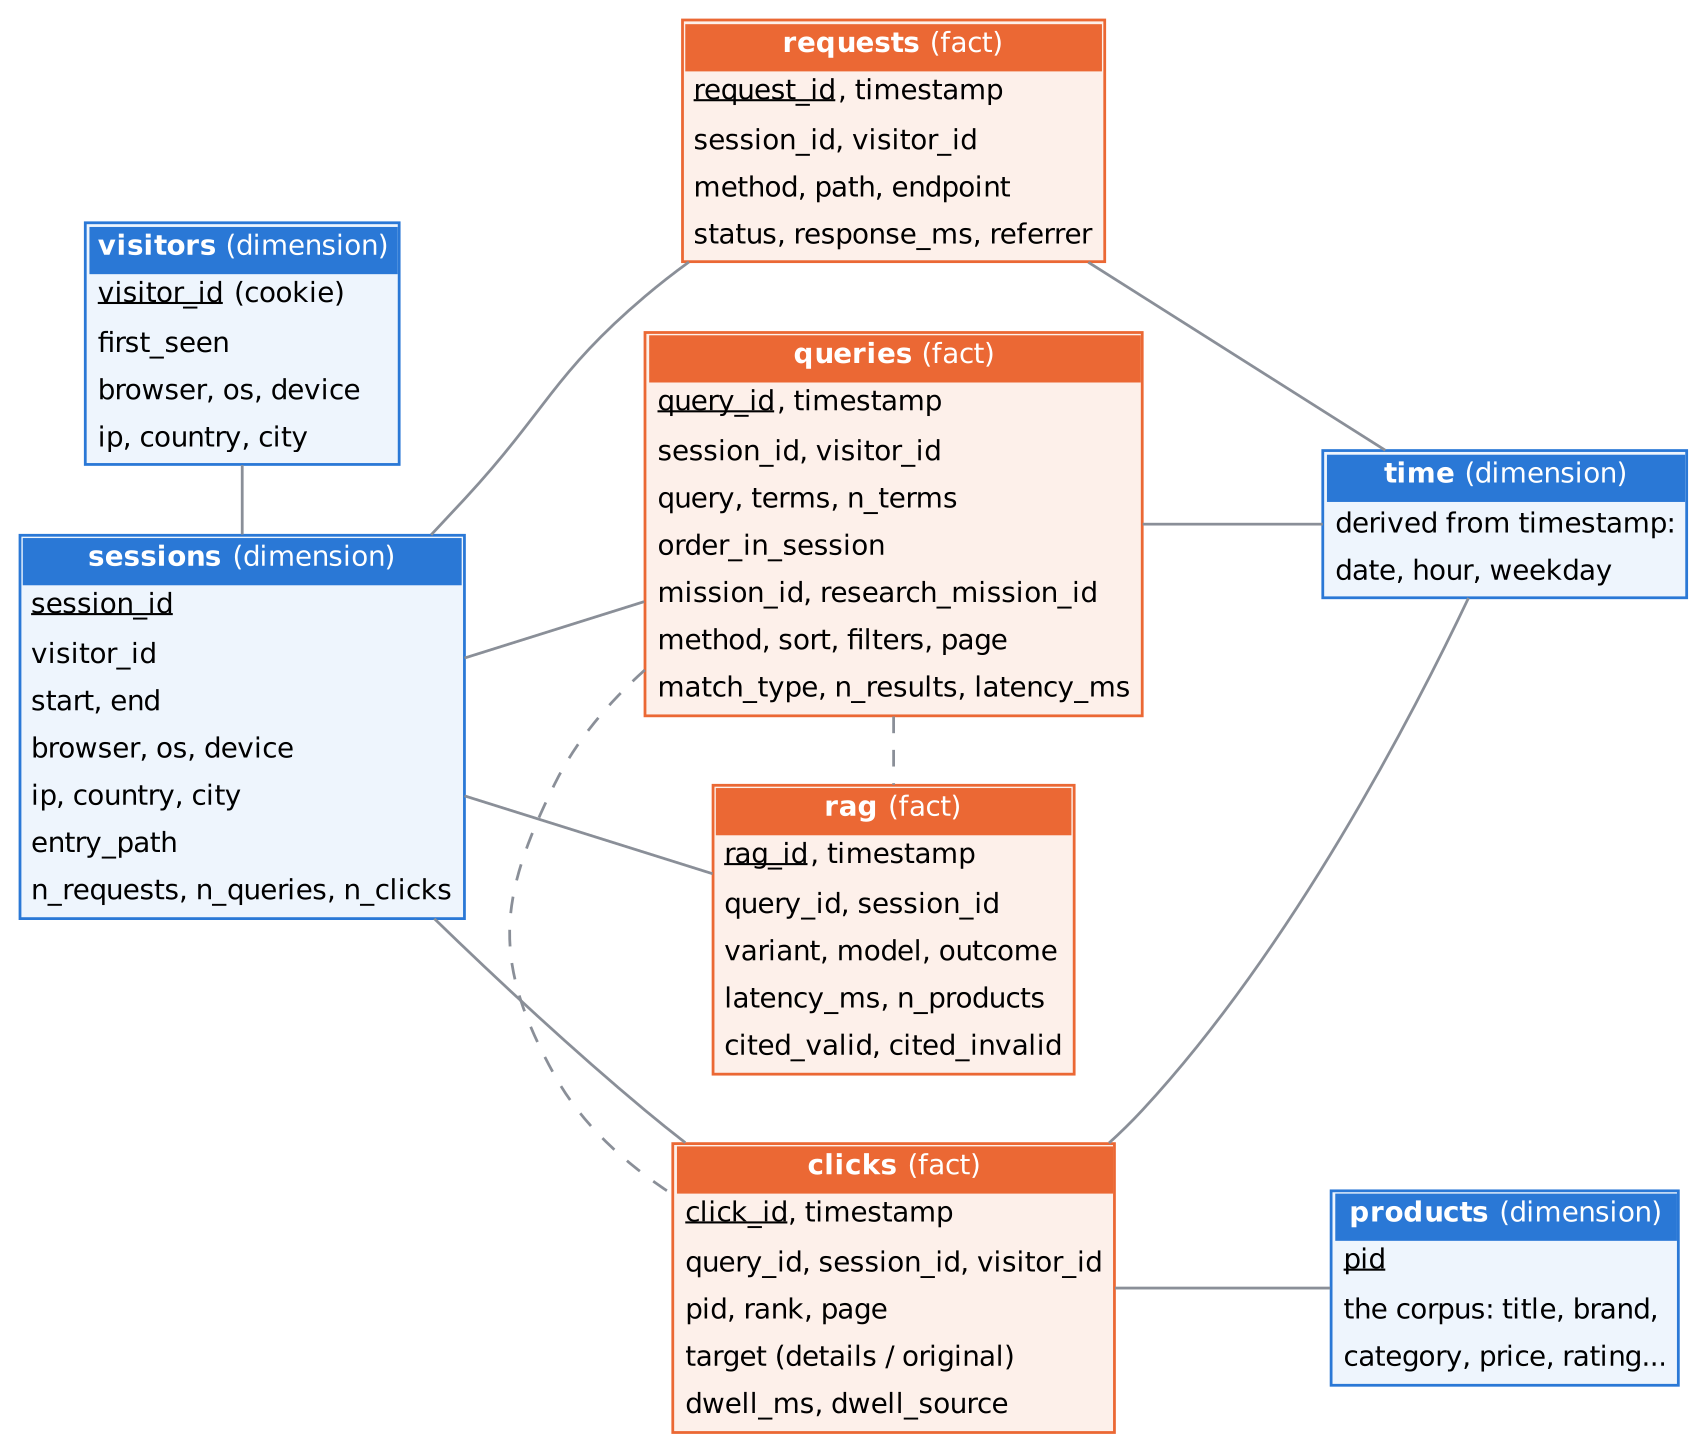
\includegraphics[width=0.88\textwidth]{figures/star_schema.png}
\caption{Star schema of the analytics data: fact tables (orange) and dimensions (blue).}
\label{fig:star}
\end{figure}

\subsection{Dashboard}
\code{/dashboard} (\code{myapp/analytics/dashboard.py}) shows the key indicators in three groups and eleven charts
(Altair, drawn in the browser with Vega-Lite, whose JavaScript files are copied in \code{static/vendor} so the
dashboard works offline). Each indicator and chart has a one-line explanation on the page. The indicators:

\begin{itemize}
\item \textbf{Traffic}: visitors, sessions, returning visitors, requests, requests per session, session length (median),
bounce rate (sessions with one request).
\item \textbf{Search}: searches, distinct queries, terms per query, searches per session, missions and searches per
mission, research missions, zero-result rate, rescued searches (spelling correction or partial match), search time
(median and 95th percentile).
\item \textbf{Results}: click-through rate (searches with a click), mean clicked rank, MRR of the clicks (mean of
1~/~rank of the first click, 0 without a click: an online version of the MRR of Part~2), median dwell time, short clicks
($<$~10~s), outbound clicks, RAG summaries.
\end{itemize}

The charts: searches and sessions per day, searches by hour, query length, clicks by rank (position bias), dwell
time, click-through rate by ranking algorithm (an online comparison of the algorithms), a session funnel (session
$\to$ search $\to$ click $\to$ original website), browser, operating system, device and country. Three tables list the
top queries with their click-through rate, the searches without a full match (words the catalogue does not have:
candidates for synonyms or new products) and the most clicked products with their mean rank and dwell time.

\textbf{Simulated traffic.} A dashboard of a new website is empty, and a few clicks by the three of us would not show
much. So we wrote \code{myapp/analytics/simulate.py}: 60 simulated visitors over 14 days, each with a browser, device and
city, 1 to 3 sessions, and missions that go from general to specific queries, sometimes with a typo, a filter or another
algorithm. On a results page a simulated user reads from the top (the chance to look at a result falls with its rank),
clicks a result that fits its goal much more often than one that does not, stays longer on it, and sometimes goes to
the original website. Every action is a real HTTP request to the application (Flask test client), so the simulation
also tests the whole tracking pipeline; only the clock, the IP and the place are set with headers that the application
accepts only in test mode. The simulated sessions are marked in the data and the dashboard says how many there are.
Figures~\ref{fig:dash1} and~\ref{fig:dash2} show the dashboard after the simulation plus our own tests. The numbers
describe the simulation, not real users: for example, the differences between algorithms in the click-through rate
come from a few dozen simulated searches each and are not a valid comparison of the rankings; with real traffic, the
same chart would be the online counterpart of the offline evaluation of Part~3.

\begin{figure}[H]
\centering
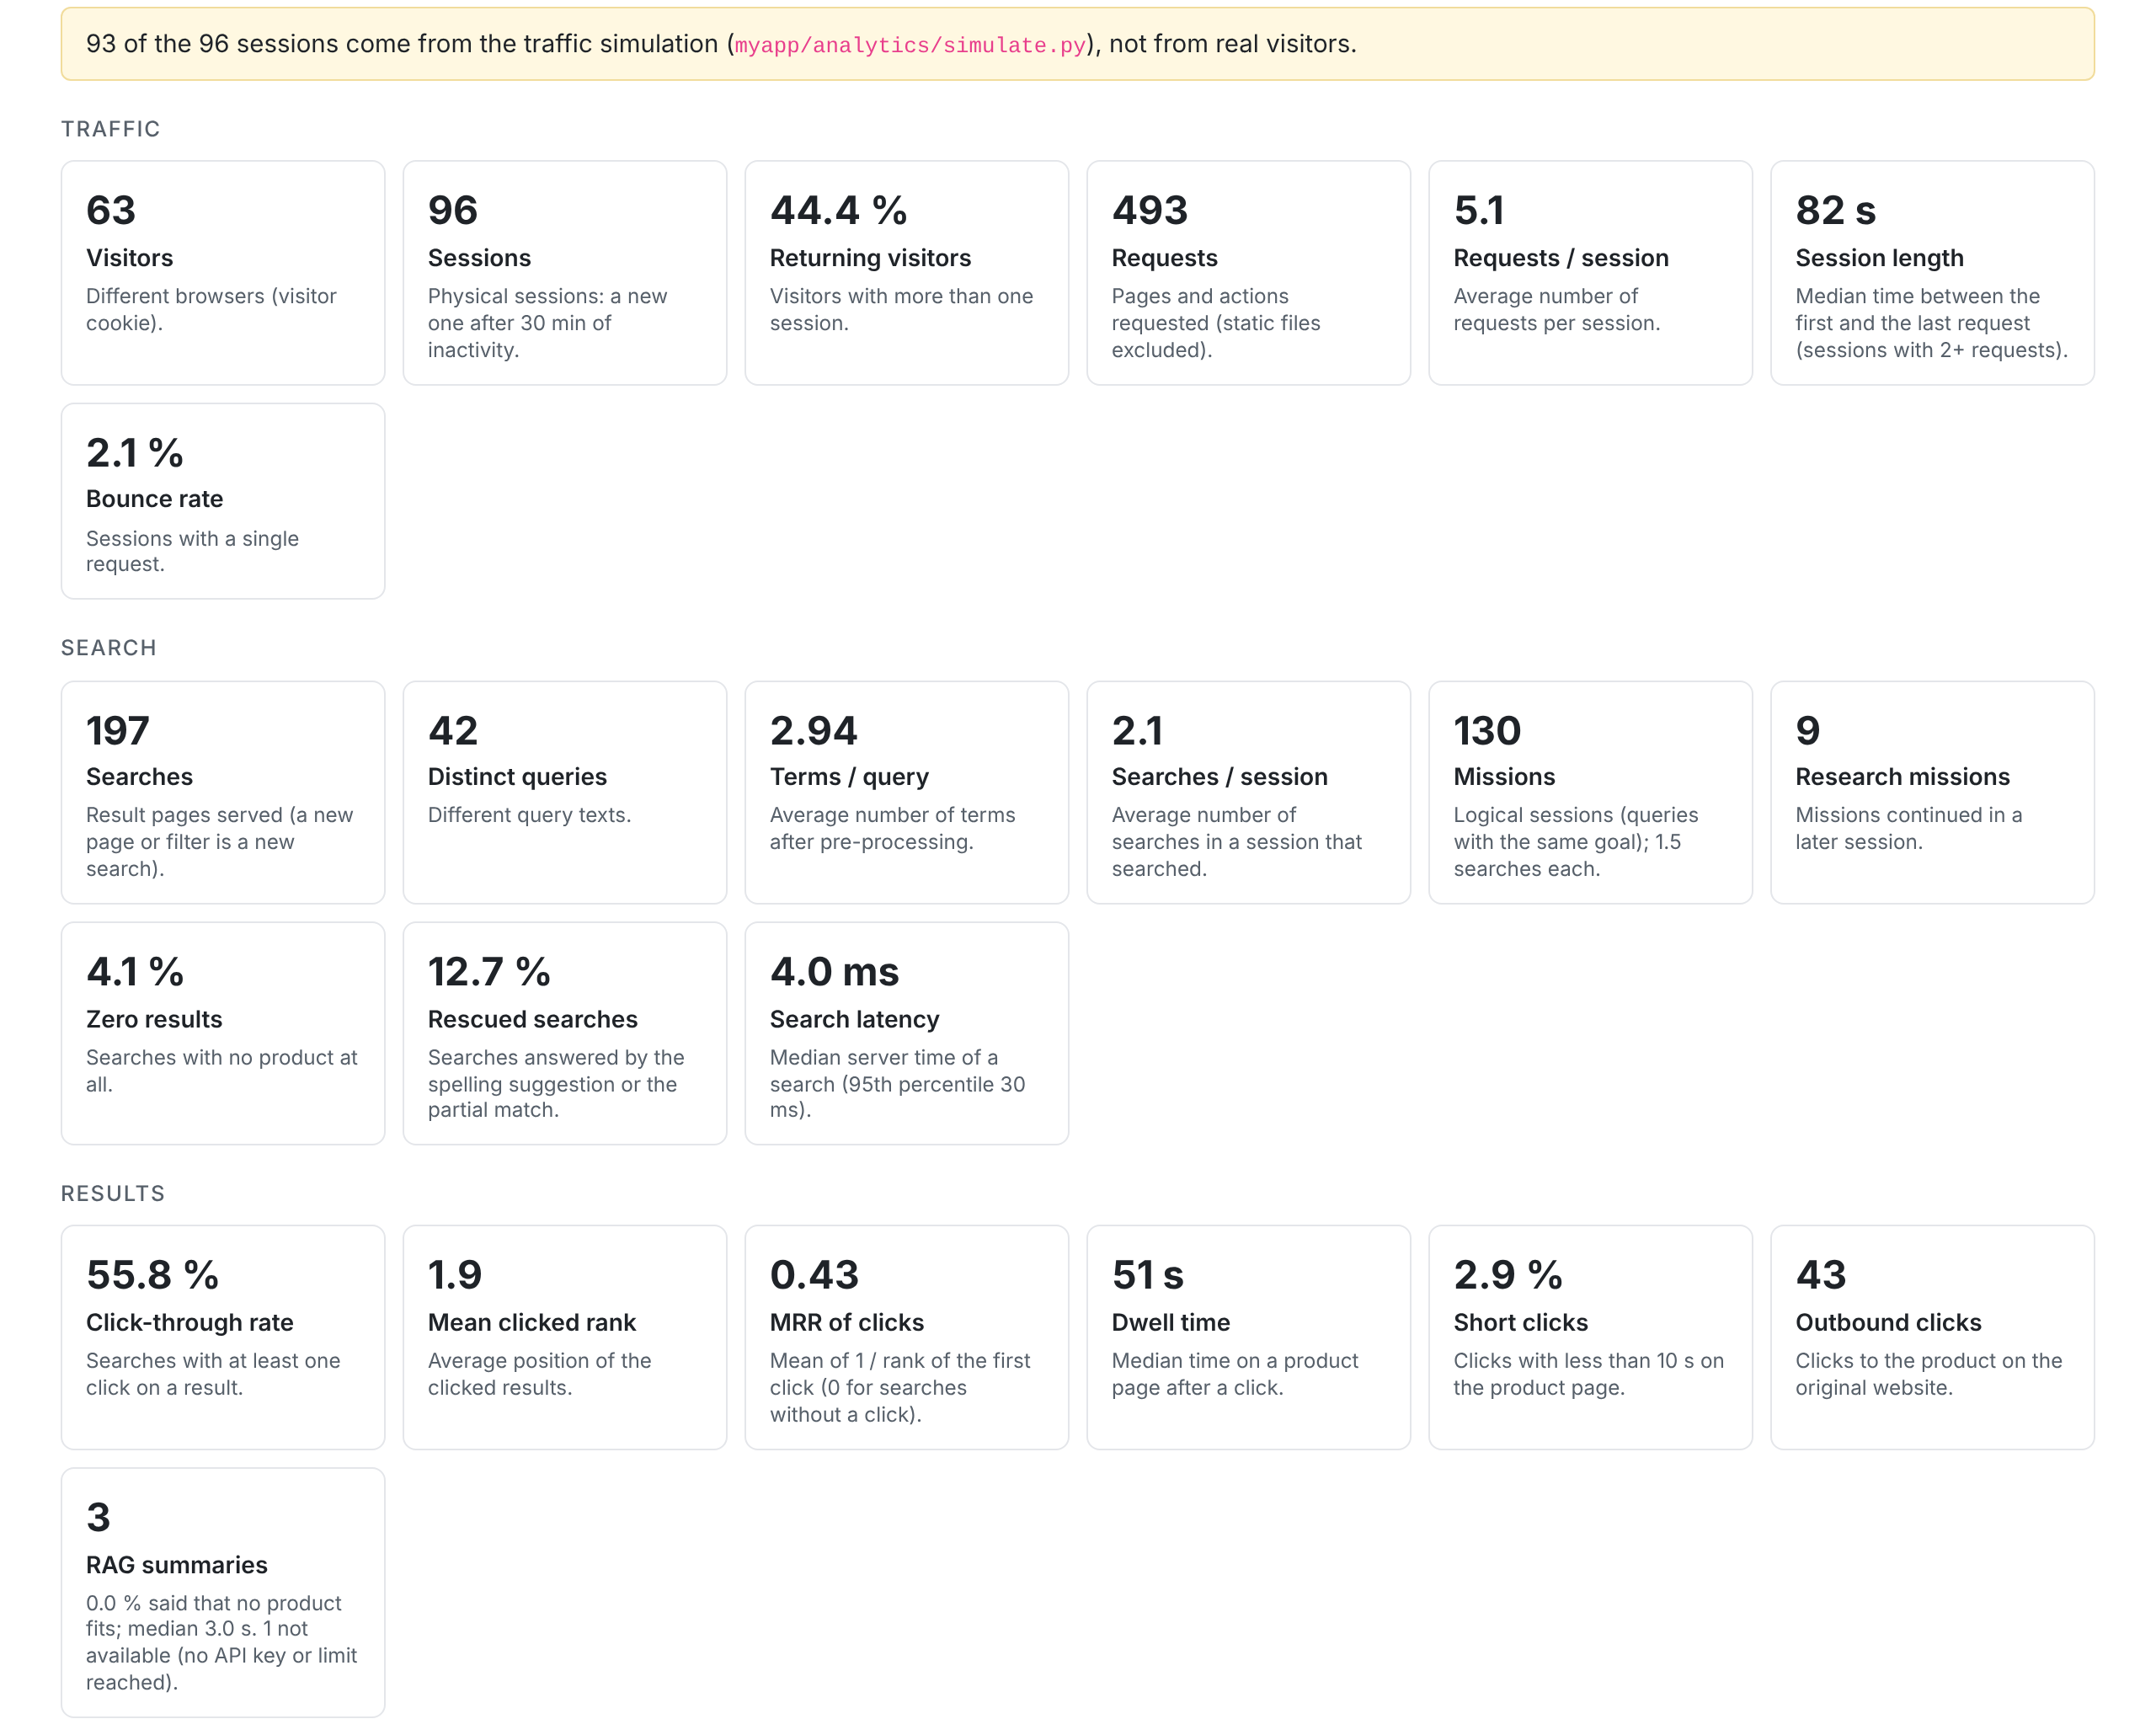
\includegraphics[width=\textwidth]{figures/dashboard_kpis.png}
\caption{Dashboard: key indicators (simulated traffic and our own tests).}
\label{fig:dash1}
\end{figure}

\begin{figure}[H]
\centering
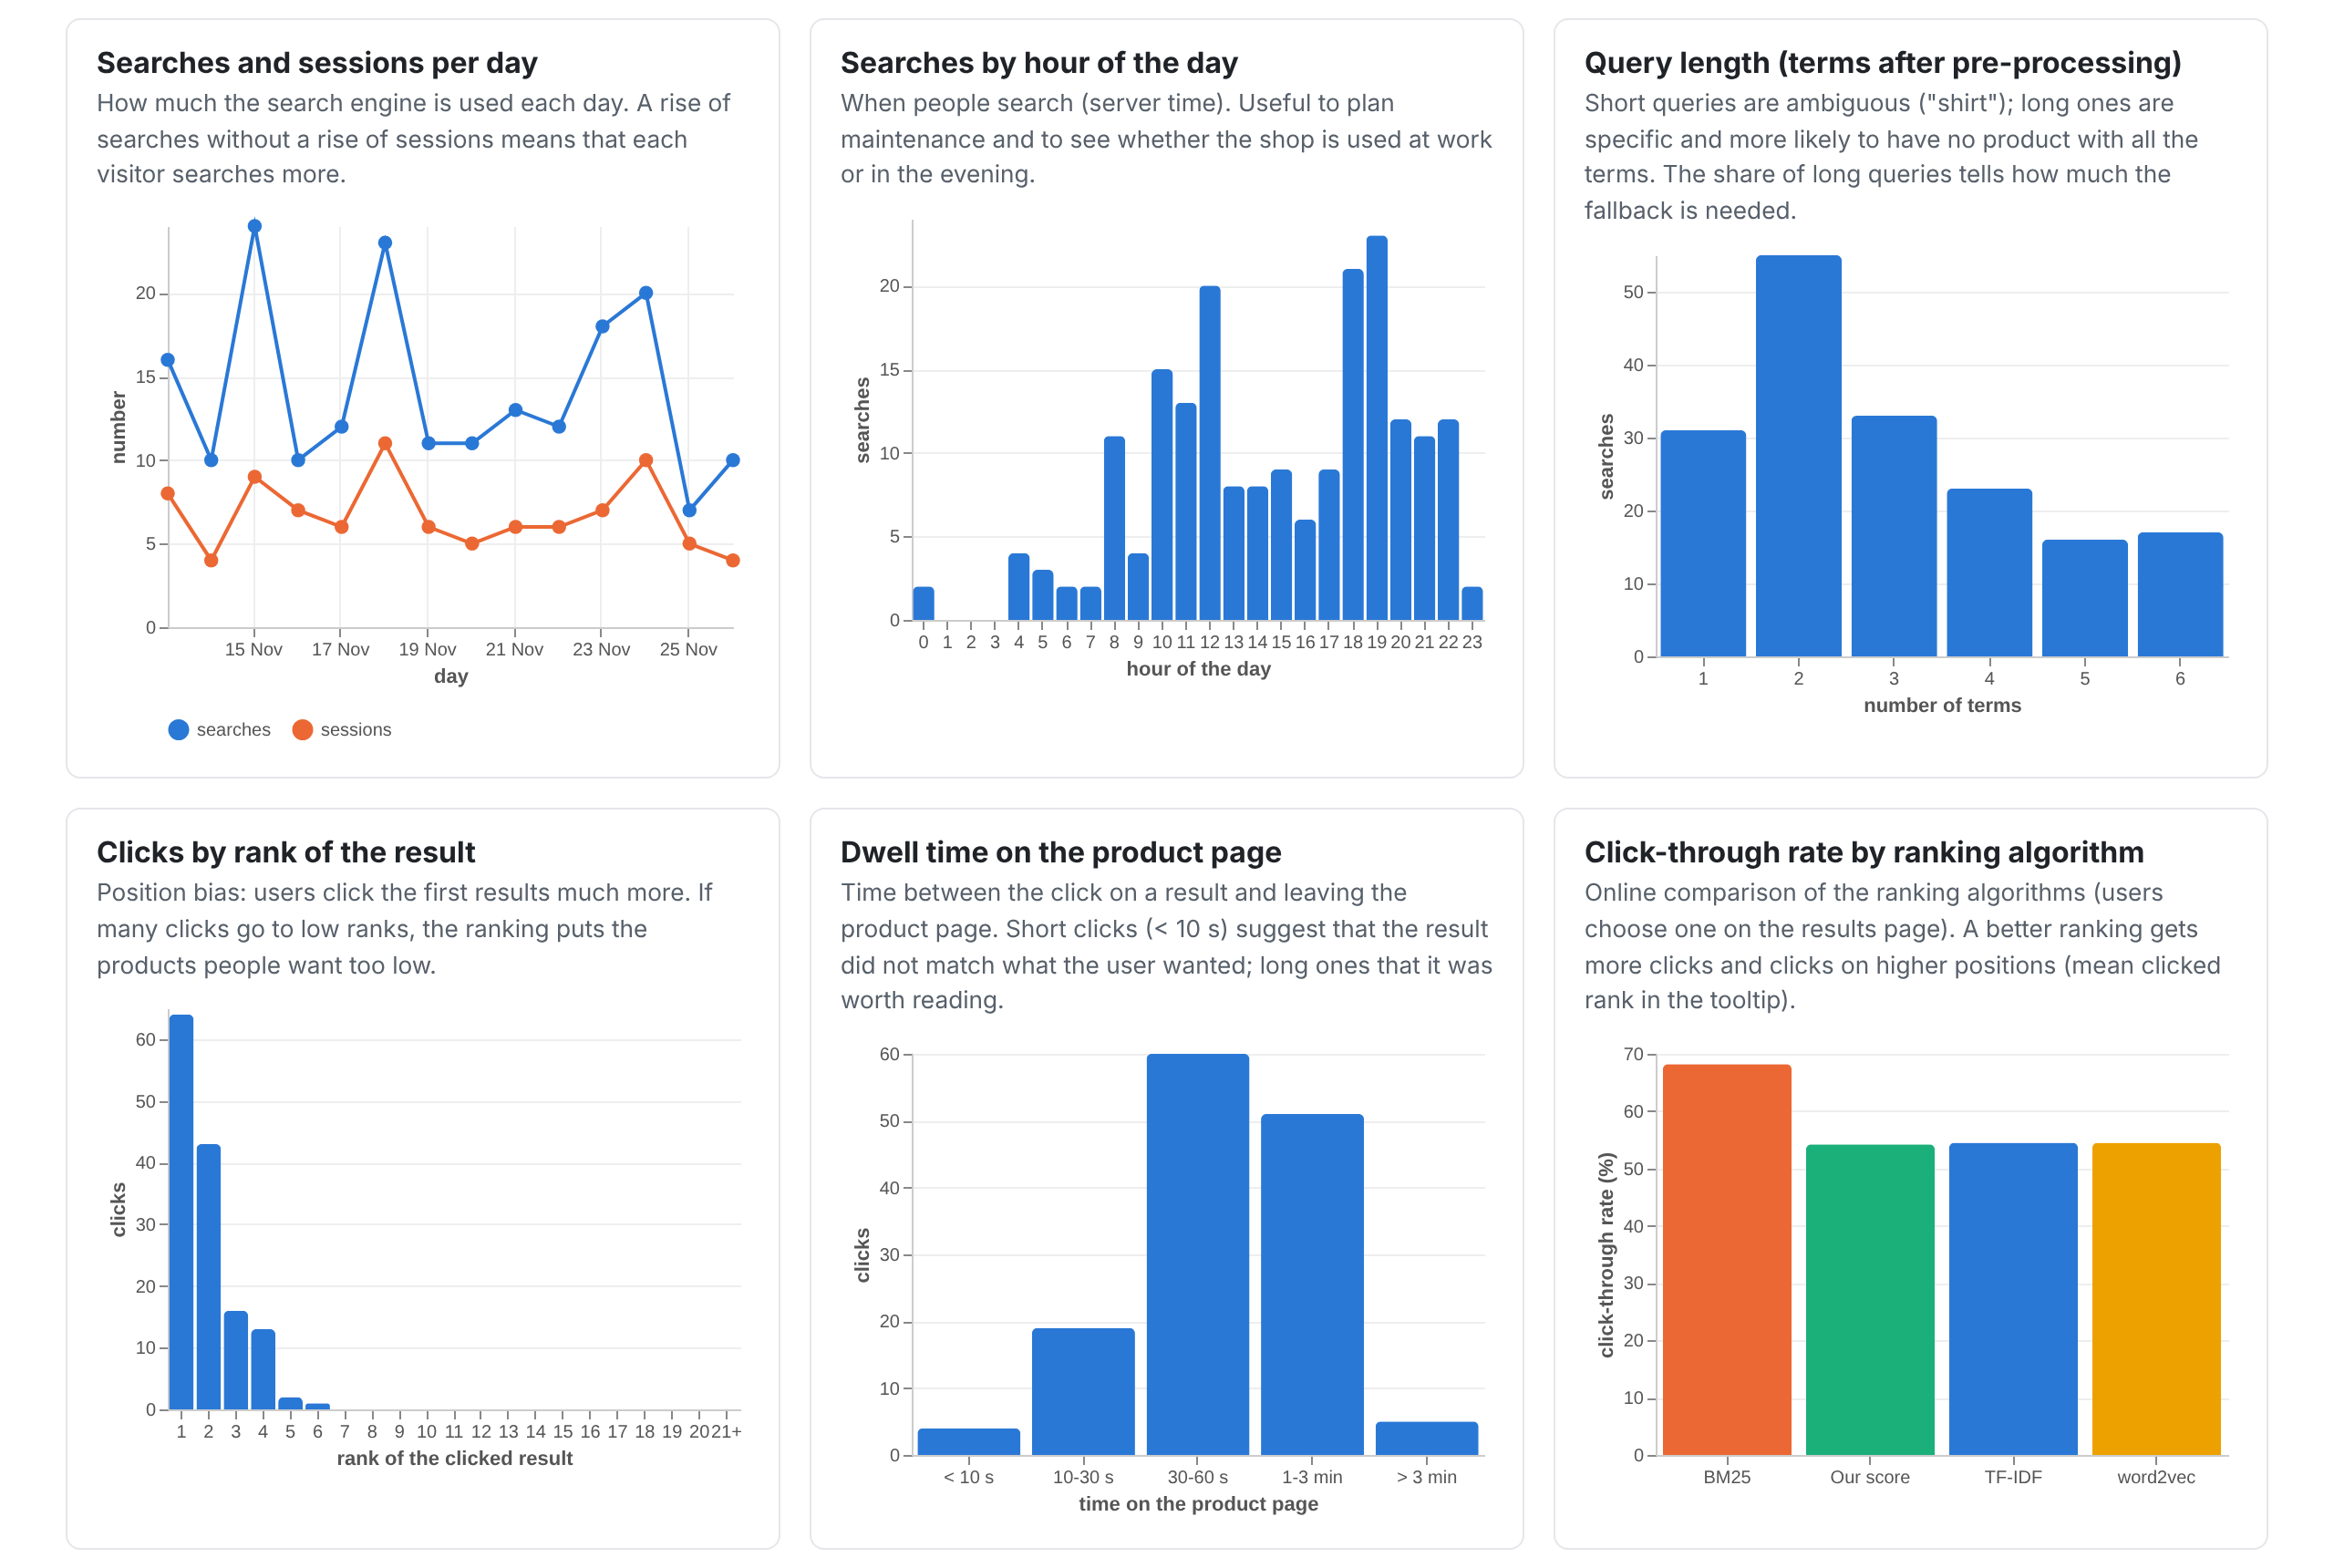
\includegraphics[width=\textwidth]{figures/dashboard_charts.png}
\caption{Dashboard: some of the charts, each with its explanation.}
\label{fig:dash2}
\end{figure}

%=====================================================================================================
\section{Assumptions and limitations}
\begin{itemize}
\item The search remains conjunctive; the fallback (spelling, partial matches) is only used when no product has all
the terms, and the page says so.
\item Keeping numbers improves the queries with numbers (Q4) but changes the lengths of the products a little; TF-IDF
gets worse on Q5 (Table~\ref{tab:numbers}). Our score, the default, is better or equal on every test query.
\item The spelling correction only uses the words of the products: a valid word that the catalogue does not have
(``laptop'') cannot be corrected, and the partial match or ``no results'' is shown.
\item The RAG evaluation uses 16 queries and automatic checks (labels, PIDs, abstention); the explanations of the
model are read by us but not scored.
\item The analytics data is kept in memory (lost at a restart unless \code{ANALYTICS\_FILE} is set) and is not
designed for many concurrent users. The dashboard shown here comes mainly from the simulation.
\item The product images are loaded from the original website; if it is not reachable, the image boxes stay empty.
\end{itemize}

\section*{Use of AI tools}
An AI assistant (Claude) only played a supporting role in our work. Before starting, we discussed
with it some ideas on how to organise the web application and how the baseline RAG could be improved. While building
the application, we asked it for help when we ran into errors we could not solve on our own, mostly to understand
and fix them. It also helped us with the code for some of the visual material of this report, such as the diagrams.
The design and implementation of the search engine, the user interface, the RAG and the analytics, as well as the
evaluations and their analysis, were done by us, and we wrote the whole report ourselves. Note that the LLM used
by our RAG is part of the application itself, not a tool that helped us do this work.

\end{document}
